\documentclass[slug=PET, room=Andreas-Schubert-Bau\,\ 424A, supervisor=Carsten\ Bittrich, coursedate=10.\ 01.\ 2020]{../../Lab_Report_LaTeX/lab_report}

\title{Postitronenemissionstomographie}
\author{Oliver Matthes, Valentin Boettcher}
\usepackage{todonotes}
\graphicspath{ {figs/} }
\usepackage{tikz}
\usepackage{pgf}
\usepackage[version=4]{mhchem}
\usepackage[ngerman]{babel}
\usepackage{subcaption}
\usepackage{amssymb}

% bib
\addbibresource{protokoll.bib}

\begin{document}
\maketitle

\section{Einleitung}
\label{sec:einl}

Dieser Versuch beschäftigt sich mit der Positronen-Emissions-Tomographie (PET), die ein
wichtiges bildgebendes Verfahren in der Medizin darstellt, um beispielsweise einen Tumore oder
allgemein Stoffwechselvorgänge sichtbar zu machen.
Dazu muss der Patient einen so genannten Tracer aufnehmen. Dabei handelt es sich um eine
radioaktive Substanz mit einer Halbwertszeit von mehreren Minuten oder Stunden, die sich an
bestimmte Geweberegionen im Körper anlagert. Bei dieser radioaktiven Substanz handelt es sich
um ein Material, das überwiegend über den \(\beta^+\) - Zerfall zerfällt.
Wie der Name des Verfahrens besagt, benötigt es für dieses Positronen. Diese werden durch eben
erwähnten \(\beta^+\) - Zerfall erzeugt:

\begin{equation}\label{eq:betazerf}
	p^+ \rightarrow n + e^+ + \nu_e
\end{equation}

Wie die Zerfallsgleichung~\ref{eq:betazerf} zeigt, zerfällt beim \(\beta^+\) - Zerfall ein Proton
in ein Neutron, das für die PET wichtige Positron und ein Elektron-Neutrino. Weswegen die
Tracer-Materialien einen Protonenüberschuss im Kern haben.
Neutrinos interagieren nur sehr selten mit Materie, weshalb die beim Zerfall entstehenden einfach
durch den Körper durchgehen und somit hier nicht interessant sind. Das Neutron verbleibt im Kern
und das Positron propagiert durch das Gewebe des Körpers mit einer Reichweite von wenigen 
Millimetern und annihiliert dann mit einem Elektron aus der Hülle eines Atoms zu zwei Photonen. 
Je besser die Auflösung dieses Verfahrens sein soll, desto kürzer darf die Reichweite der 
Positronen sein, das heißt: Je näher sie am Entstehungsort annihilieren, desto besser.

\begin{equation}\label{eq:annihi}
	e^+ + e^- \rightarrow \gamma + \gamma
\end{equation}

Die entstehenden Photonen haben stets die gleiche Energie. Die Ruhemasse von Elektron und Positron
beträgt \(\SI{1022}{\kilo\electronvolt}\) und teilt sich bei der Paarvernichtung gleichmäßig auf 
die Photonen auf, sodass diese ergo eine Energie von \(E_\gamma = \SI{511}{\kilo\electronvolt}\).
Da die Annihilation in Ruhe stattfindet und Energie und Impulserhaltung gilt, schließen die beiden
Photonen einen Winkel von \(180^\circ\) ein, bewegen sich also antiparallel.\\

Um den Beobachtungsort sind in einem Ring (in diesem Versuch nur zwei gegenüberliegende)
Detektoren angebracht, die die entstandenen Photonen registrieren.
Allerdings können zum Beispiel durch andere Zerfallsprozesse natürlich auch andere Photonen
entstehen, die die Messungen stören. Um solche zufällige Koinzidenzen möglichst gering zu halten,
müssen die eintreffenden Lichtquanten bestimmte Kriterien erfüllen:\\
Wie eben beschrieben haben die Photonen immer die gleiche Energie, sodass Photonen, die nicht in
ein Energiefenster passen, nicht berücksichtigt werden. Des Weiteren haben die Detektoren einen
bestimmten Abstand zu einander, was bedeutet, dass die Photonen mit einer maximalen zeitlichen
Differenz von Detektorabstand geteilt durch Lichtgeschwindigkeit eintreffen müssen, sofern sie
innerhalb des PET erzeugt wurden.\\

Die Zählrate der wahren Koinzidenzen, also der für uns interessanten ergibt sich folgendermaßen:

\begin{equation}\label{eq:wahrkoinz}
	\dot N_K = \qty(\frac{\Omega_{min}}{2 \pi}) \cdot P_\beta A \cdot \epsilon_1 \epsilon_2
\end{equation}

\begin{conditions}
	\Omega_{min} & Raumwinkelelement des von der Quelle am weitesten entfernten Detektors\\
	P_\beta & Zerfallswahrscheinlichkeit des Nuklids für \(\beta^+\) - Zerfall\\
	A & Aktivität der Quelle\\
	\epsilon_1/\epsilon_2 & intrinsische Nachweiseffektivitäten der Detektoren
\end{conditions}

Die Detektoren, die für die PET verwendet werden, sind Szintillationsdetektoren. Einfach
beschrieben absorbiert ein Szintillator ein eintreffendes Photon und wandelt dieses in Photonen
mit einer anderen Wellenlänge, die meist im sichtbaren oder ultravioletten Bereich liegt, um.
Dabei dient das Szintillatormaterial, das in diesem Versuch aus Kristallen besteht (es gibt
aber auch weitere Szintillatortypen, beispielsweise organische, die mit Plastik als Material
arbeiten) auch als Lichtleiter.
Hinter dem Kristall befindet sich eine Photokathode, die die eintreffenden Photonen über den 
Photoelektrischen Effekt in Elektronen umwandeln. Da die durch die Photonen herausgelösten
Elektronen sehr wenige sein können, zu wenige, um ein Signal zu messen, ist nun noch ein
Photomultiplier angeschlossen, der die Elektronen mittels Hochspannung beschleunigt und die
Anzahl der Elektronen vervielfältigt. Diese Vervielfältigung funktioniert über Dynoden. Auf diese
prallen die Elektronen auf und lösen mehrere Sekundärelektronen heraus. Durch
Hintereinanderreihung von mehreren Dynoden, steigt die Elektronenanzahl exponentiell an.\\

Um mit Hilfe der Szintillatoren auf die Energie sowie den Ort der im Detektor erzeugten Photonen
schließen zu können, ist ein Szintillatorkristall von vier Photomultipliern unterschiedlich tief
eingeschnitten. Diese Art von Detektoren nennt sich Blockdetektoren. In diesem Versuch ist der
Kristall vor den vier Photomultipliern in einer 8 x 8 - Matrix unterteilt.
Die so aufgenommenen Amplituden sind aufsummiert proportional zu der Energie, die von den
Photonen im Detektor deponiert wurde. Bildet man den Schwerpunkt der Amplituden kann man
den Ort, an dem die Photonen mit dem Kristall wechselwirkten, bestimmen.\\

Bei diesem Verfahren wird also eine zweidimensionale Abbildung, eine Quellverteilung, die man 
untersuchen will, auf eine eindimensionale Funktion, die eine Intensitätsverteilung beschreibt, 
projiziert.
Dieser Vorgang wird mathematisch durch die Radon-Transformation beschrieben. Diese Transformation
projiziert eine zweidimensionale Funktion auf eine Gerade \(s\), die durch den Koordinatenursprung
läuft und einen Winkel \(\vartheta\) mit der x-Achse einschließt.
Die Projektion ordnet dabei den auf der Projektionsgeraden \(s\) befindlichen Punkten ein
Linienintegral \(p(s, \vartheta)\) zu:

\begin{equation}\label{eq:linienint}
	p(s, \vartheta) = \int_{-R_I}^{+R_I} f_I(s \cdot \cos \vartheta - t \cdot \sin \vartheta, s \cdot \sin\vartheta + t \cdot \cos\vartheta)
\end{equation}

Wobei folgende Beziehungen genutzt wurden:

\begin{align}
	s = x \cdot \cos\vartheta + y \cdot \sin\vartheta \\
	x = s \cdot \cos \vartheta - t \cdot \sin \vartheta \\
	y = s \cdot \sin\vartheta + t \cdot \cos\vartheta \\
	R_I = \sqrt{x^2 + y^2}
\end{align}

Stellt man die Funktion \(p(s, \vartheta)\) zweidimensional dar, erhält man ein so genanntes
\emph{Sinogramm}.

\section{Auswertung}
\label{sec:ausw}

\subsection{Theoriebeispiel}
\label{sec:theobei}
Zur Verbesserung des verst\"andnisses der Projektions- und
Rekonstruktionsprozesse, werden diese hier anhand eines einfachen
Beispiels nachvollzogen.

\begin{figure}[htp]
  \centering
  \begin{subfigure}[t]{.25\textwidth}
    \centering
    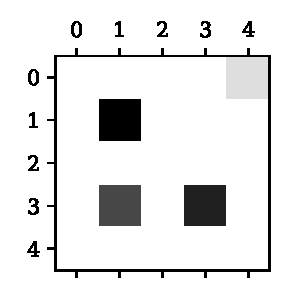
\includegraphics[width=.6\textwidth]{../auswertung/figs/theory/source.pdf}
    \caption{Ausgangsmatrix}
    \label{fig:theory-source}
  \end{subfigure}
  \begin{subfigure}[t]{.25\textwidth}
    \centering
    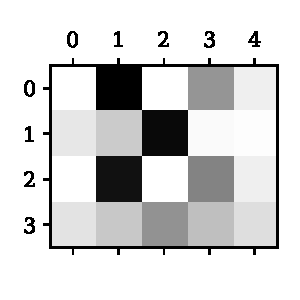
\includegraphics[width=.6\textwidth]{../auswertung/figs/theory/projection.pdf}
    \caption{Sinogram}
    \label{fig:theory-projection}
  \end{subfigure}
  \begin{subfigure}[t]{.25\textwidth}
    \centering
    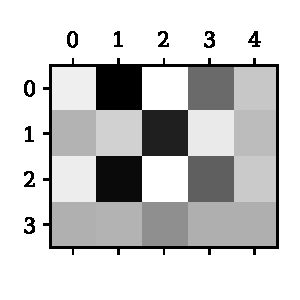
\includegraphics[width=.6\textwidth]{../auswertung/figs/theory/convoluted.pdf}
    \caption{Gefiltertes Sinogram}
    \label{fig:theory-convoluted}
  \end{subfigure}
  \begin{subfigure}[t]{.25\textwidth}
    \centering
    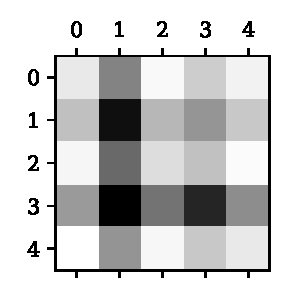
\includegraphics[width=.6\textwidth]{../auswertung/figs/theory/rec_simple.pdf}
    \caption{Einfache R\"uckprojektion}
    \label{fig:theory-rec_simple}
  \end{subfigure}
  \begin{subfigure}[t]{.25\textwidth}
    \centering
    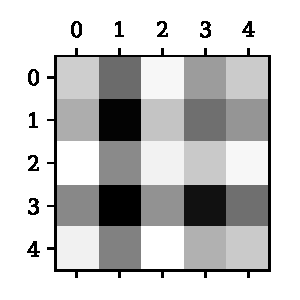
\includegraphics[width=.6\textwidth]{../auswertung/figs/theory/rec_filtered.pdf}
    \caption{Gefilterte R\"uckprojektion}
    \label{fig:theory-rec_filtered}
  \end{subfigure}
  \caption[Graustufendarstellung der
  Beispielmatrizen]{Graustufendarstellung der Matrizen aus den
    Teilschritten des Beispiels. Es wurden jeweils die Matrixelemente
    in das Interval \([0,1]\) reskaliert.}
  \label{fig:graubei}
\end{figure}

Im ersten Schritt wird die Projektion~\ref{fig:theory-projection} des
Ausgangsbildes~\ref{fig:theory-source} aus Verschiedenen Winkeln
berechenet. Dabei wurden die diagonalen entsprechend gewichtet.

\begin{equation}
  \label{eq:proj}
  \mathfrak{M}_0 =
  \begin{pmatrix}
    0 & 0 & 0 & 0 & 2\\
    0 & 9 & 0 & 0 & 0\\
    0 & 0 & 0 & 0 & 0\\
    0 & 7 & 0 & 8 & 0\\
    0 & 0 & 0 & 0 & 0\\
  \end{pmatrix}
  \implies
  \left(
    \begin{array}{ccccc|c}
      0. & 16. & 0. & 8. & 2 & 0^\circ\\
      2.73 & 4.95 & 15.47 & 0.68 & 0.28 & 45^\circ\\
      0. & 15. & 0. & 9. & 2. & 90^\circ\\
      3.12 & 5.24 & 8.19 & 5.85 & 3.51 & 135^\circ\\
    \end{array}\right) = \mathfrak{P}_0
\end{equation}

Ein gefiltertes Sinogram~\ref{fig:theory-convoluted} ergibt sich durch
Faltung der Zeilen von \(\mathfrak{M}_0\) mit
\(F = \mqty(-.1 & .25 & -.1)\).

\begin{equation}
  \label{eq:filter}
  \mathfrak{M}_1 = \mathfrak{M}_0 * F =
  \begin{pmatrix}
    -1.6 & 4. & -2.4 & 1.8 & -0.3\\
    0.188 & -0.583 & 3.304 & -1.405 & 0.002\\
    -1.5 & 3.75 & -2.4 & 2.05 & -0.4\\
    0.256 & 0.179 & 0.938 & 0.293 & 0.292\\
  \end{pmatrix}
\end{equation}

Die R\"uckprojektion des Einfachen sinogramms
ergib~\ref{fig:theory-rec_simple}.

{\footnotesize
\setlength{\arraycolsep}{2.5pt}

\begin{align}
  \label{eq:simplerepr}
  \overbrace{\begin{pmatrix}
      0. & 16. & 0. & 8. & 2.\\
      0. & 16. & 0. & 8. & 2.\\
      0. & 16. & 0. & 8. & 2.\\
      0. & 16. & 0. & 8. & 2.\\
      0. & 16. & 0. & 8. & 2.\\
    \end{pmatrix}}^{0^\circ} & + \frac{1}{2}\overbrace{\begin{pmatrix}
      15.864 & 8.408 & 0.837 & 0.287 & 0.076\\
      12.636 & 15.864 & 8.408 & 0.837 & 0.287\\
      6.569 & 12.636 & 15.864 & 8.408 & 0.837\\
      2.78 & 6.569 & 12.636 & 15.864 & 8.408\\
      0.737 & 2.78 & 6.569 & 12.636 & 15.864\\
    \end{pmatrix}}^{45^\circ} \nonumber \\ + \overbrace{\begin{pmatrix}
      2. & 2. & 2. & 2. & 2.\\
      9. & 9. & 9. & 9. & 9.\\
      0. & 0. & 0. & 0. & 0.\\
      15. & 15. & 15. & 15. & 15.\\
      0. & 0. & 0. & 0. & 0.\\
    \end{pmatrix}}^{90^\circ} &+ \frac{1}{2}\overbrace{\begin{pmatrix}
      0.842 & 3.172 & 7.12 & 9.283 & 8.966\\
      3.172 & 7.12 & 9.283 & 8.966 & 9.886\\
      7.12 & 9.283 & 8.966 & 9.886 & 8.003\\
      9.283 & 8.966 & 9.886 & 8.003 & 3.569\\
      8.966 & 9.886 & 8.003 & 3.569 & 0.948\\
    \end{pmatrix}}^{135^\circ}\nonumber \\
  & = \begin{pmatrix}
    10.353 & 23.79 & 5.978 & 14.785 & 8.521\\
    16.904 & 36.492 & 17.845 & 21.902 & 16.087\\
    6.844 & 26.959 & 12.415 & 17.147 & 6.42\\
    21.031 & 38.768 & 26.261 & 34.933 & 22.988\\
    4.852 & 22.333 & 7.286 & 16.102 & 10.406\\
  \end{pmatrix} = \mathfrak{M}_1
\end{align}}

Aus dem gefilterten Sinogram ergibt sich auf \"ahnliche
Weise~\ref{fig:theory-rec_filtered}
{\footnotesize
\setlength{\arraycolsep}{2.5pt}

\begin{align}
  \label{eq:simplerepr}
  \overbrace{\begin{pmatrix}
      -1.6 & 4. & -2.4 & 1.8 & -0.3\\
      -1.6 & 4. & -2.4 & 1.8 & -0.3\\
      -1.6 & 4. & -2.4 & 1.8 & -0.3\\
      -1.6 & 4. & -2.4 & 1.8 & -0.3\\
      -1.6 & 4. & -2.4 & 1.8 & -0.3\\
    \end{pmatrix}}^{0^\circ} & + \frac{1}{2}\overbrace{\begin{pmatrix}
      3.165 & 0.261 & -1.305 & -0.012 & 0.001\\
      1.076 & 3.165 & 0.261 & -1.305 & -0.012\\
      -0.407 & 1.076 & 3.165 & 0.261 & -1.305\\
      0.182 & -0.407 & 1.076 & 3.165 & 0.261\\
      0.051 & 0.182 & -0.407 & 1.076 & 3.165\\
    \end{pmatrix}}^{45^\circ} \nonumber \\ +
  \overbrace{\begin{pmatrix}
      -0.4 & -0.4 & -0.4 & -0.4 & -0.4\\
      2.05 & 2.05 & 2.05 & 2.05 & 2.05\\
      -2.4 & -2.4 & -2.4 & -2.4 & -2.4\\
      3.75 & 3.75 & 3.75 & 3.75 & 3.75\\
      -1.5 & -1.5 & -1.5 & -1.5 & -1.5\\
    \end{pmatrix}}^{90^\circ} &+ \frac{1}{2}\overbrace{\begin{pmatrix}
      0.069 & 0.258 & 0.351 & 0.646 & 0.972\\
      0.258 & 0.351 & 0.646 & 0.972 & 0.759\\
      0.351 & 0.646 & 0.972 & 0.759 & 0.486\\
      0.646 & 0.972 & 0.759 & 0.486 & 0.295\\
      0.972 & 0.759 & 0.486 & 0.295 & 0.079\\
    \end{pmatrix}}^{135^\circ}\nonumber \\
           &= \begin{pmatrix}
             -0.383 & 3.86 & -3.277 & 1.717 & -0.214\\
             1.117 & 7.808 & 0.104 & 3.683 & 2.123\\
             -4.028 & 2.461 & -2.732 & -0.09 & -3.11\\
             2.564 & 8.032 & 2.267 & 7.375 & 3.728\\
             -2.589 & 2.97 & -3.861 & 0.985 & -0.178\\
           \end{pmatrix} = \mathfrak{M}_2
\end{align}
}

Es ist zu erkennen, das in beiden rekonstruktionen die starken Signale
\((1,1),\,(3,1),\,(3,3)\) klar zu identifizerien, wenngleich die
Unterschiede in der signalst\"arke nicht im urspr\"unglichen
Verh\"altniss stehen. Die gefilterte R\"uckprojektion weist in den
Randfeldern und im Mittleren Feld einen h\"oheren Kontrast auf,
erzeugt aber dennoch nur ein geringf\"ugig besseres und in manchen
Bereichen (Ecken) sogar ein schlechteres Bild. Das schwache Signal
\((0,4)\) wurde in beiden F\"allen nicht rekonstruiert. F\"uhrt man
die Rechnung ohne diesen Punkt aus, ergibt sich kaum ein
Unterschied. Schwache Signale werden also nicht gut reproduziert.

\newpage
\section{Verzeichnisse}
\label{sec:literatur}

\listoffigures

\listoftables

\printbibliography
\end{document}
